\chapter{共識演算法}\label{se_3}

\section{共識流程}\label{se_3} 
我們的目標是設計一個每個回合只須執行兩個步驟的BFT演算法。更明確地說,在一個步驟中,一個節點可以依序做以下事情: (一)廣播訊息。(二)接收訊息。(三)做本地端的運算(Local Computation)。在我們提出的BFT演算法中,每個回合包含兩個步驟:在第一個步驟中,共識演算法會用依序循環(Round-Robin)的方法在每回合選出一名提議者。只有該名提議者可以在該回合廣播提議。在第二個步驟中,所有節點會投票(廣播訊息)和收集其他節點的選票(接收訊息)。我們的演算法受到MSIG-BFT \cite{chen2018msig}的啟發,MSIG-BFT是一個每回合需要執行三個步驟的共識演算法。 與MSIG-BFT演算法一樣,如果網絡狀況不佳,提議者有可能會被禁止廣播提議。下面將詳細描述這兩個步驟。
%\begin{figure}
\centering
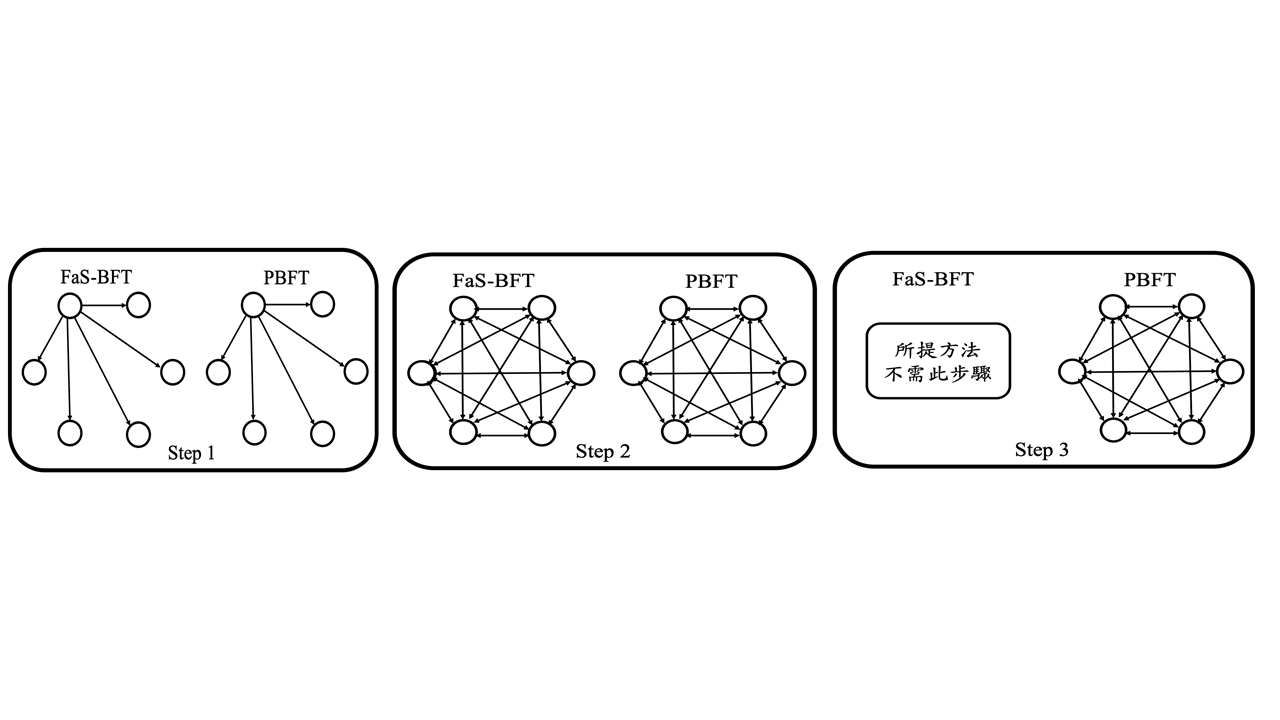
\includegraphics[scale=0.45]{images/31.png}
\caption{TwoStepBFT演算法流程圖}
\label{i:byz-latency}
\end{figure}
\subsection{Propose}\label{se_3} 
第一步:在第一個步驟中的主要目標為讓提議者廣播提議。我們稱這個廣播的訊息為Proposal訊息。 若$p$為一個Proposal訊息,則我們用$p.B$ 代表該Proposal訊息中的提議值。舉例來說,在區塊鏈中,$p.B$ 可能是該提議者產生的區塊。另外我們用$p.R$ 代表該Proposal訊息被產生的回合數。舉例來說,若$p$是第二回合的提議者廣播的Proposal訊息,則$p.R = 2$。第一步驟的虛擬碼如圖Algorithm 1 所示。我們會在解釋完第二個步驟後詳細討論第一個步驟。
\begin{algorithm}
%  \SetAlgoNoLine
  \caption{Propose:從節點$u$來觀察}
  \KwIn{節點$u$具有初始值$bin$,以及上一回合的票集合$loclset(r-1)$}
  $ldr$ = 在$r$回合的廣播提議者

  \If{$u$=$ldr$}{
   製作一個提案$p$

   $p.R$ $\gets$ $r$
   
   // 確認$p.B$並且將$p$廣播給所有節點

   \If{$r$=1}{

   $p.B$ $\gets$ $bin$ 並且將$p$廣播給所有節點

    }
  
  \ElseIf{$|loclset(r-1)|$ $\ge$ 4$f$+1}{
    
    \If{$\exists$一個$b$,且$b$$\ne$ $\varnothing$且|{$v$|$v$ $\in$$loclset(r-1)$,$v,B$=$b$ }|$\ge$ 2$f$+1}{
    $b$可以為任何值
    $p.B$ $\gets$ $b$並且將$p$廣播給所有節點
    }
    \Else{

    $p.B$ $\gets$ $bin$並且將$p$廣播給所有節點
    }

    }
    
}
   
\end{algorithm}

\subsection{Vote}\label{se_3} 
第二步:第二個步驟的主要目標為讓所有節點對接收到的Proposal訊息$p$投票,並在收到足夠多選票的情況下,提交(Commit)提議值(在區塊鏈的應用中,提交代表將區塊鏈接在區塊鏈的尾端)。為了實現這個目標,一旦節點$u$ 收到Proposal訊息$p$,則節點$u$ 首先驗證提議值$p.B$的正確性。舉例來說,在區塊鏈的應用中,節點$u$會檢查提議值$p.B$ 是否為一個合法的區塊。如果提議值$p.B$通過驗證,則$u$會廣播一個包含$p.B$ 的投票訊息(選票)。每個節點在一回合中最多只能廣播一個投票訊息。如果節點在某個預定的時間$TOcommit$內收到$4f+ 1$個投票訊息,並且這些$4f+1$的投票訊息包含相同的非空(Non-empty)提議值$b$,則節點提交提議值$b$。另一方面,如果節點$u$在時間$TOcommit$到之前無法提交,那麼節點$u$需要紀錄這個回合廣播的投票訊息中的候選值$b$,並進入下個回合。更明確地說,若$b$是在第$i$個回合中,由$u$廣播的投票訊息中的候選值,則在第$i$ + 1個回合中,如果$u$在另一個的時間$TOvote$到期之前,仍然無法收到有效的Proposal訊息,則$u$廣播的投票訊息會包含提議值$b$。值得注意的是,在第一個回合時,如果$u$ 在$TOvote$到期之前無法收到有效的Proposal訊息,則$u$ 廣播的投票訊息會包含空提議值 $\varnothing$。每當進入下一回合時,上述兩個預定時間($TOcommit$ 與$TOvote$)的長度會加倍。若 $v$ 為一個投票訊息,我們使用$p.R$和$p.B$表示$v$ 被產生的回合數和$v$中包含的提議值。第二步驟的虛擬碼如圖Algorithm 2 所示。
\begin{algorithm}
%  \SetAlgoNoLine
  \caption{Vote:從節點$u$來觀察}
    // 確認$v.B$並且將$v$廣播給所有節點



\If{在$TOvote$到期之前,$u$在第$r$回合收到一個合法的Proposal $p$}{
  $v.B$ $\gets$ $p.B$並且將$v$廣播給所有節點
}

\Else{

\If{$r$=1}{
  
  $v.B$ $\gets$ $\varnothing$
}
\Else{ 
  $v'$ $\gets$ $u$在$r$-1回合廣播的投票vote
  $v.B$ $\gets$ $v'.B$
}
    廣播$v$   
}
\If{在$TOcommit$到期之前,$u$在第$r$回合收到4$f$+1張vote訊息且包含一樣的 $b$且$b$ $\neq$ $\varnothing$}{
  
 Commit $b$

}
\Else{
進到$r$+1回合
}
  
\end{algorithm}

\subsection{Commit}\label{se_3}
Commit 階段是各節點根據上一個步驟的投票結果,判斷是否可以進行提交區塊如果存在 $lockset(h,r)$ = $b$,則提交區塊 $b$ 至區塊鏈上完成高度$h$的共識。如果 $lockset(h,r)$ = $b$不存在,則進入第一階段Propose且進入$r+1$回合。

\section{Timeout}\label{se_3}

共識中的Timeout會隨著$R$的增加進行指數型成長其成長公式為: 

$Timeout_X,_R$ = $Timeout_X$ * $TimeoutFactor^R$

其中$X$為$TOvote$或$TOcommit$,$Timeout$的起始值其值為5秒,$TimeoutFactor$預設則為2。 

\begin{figure}[!htbp]
\centering
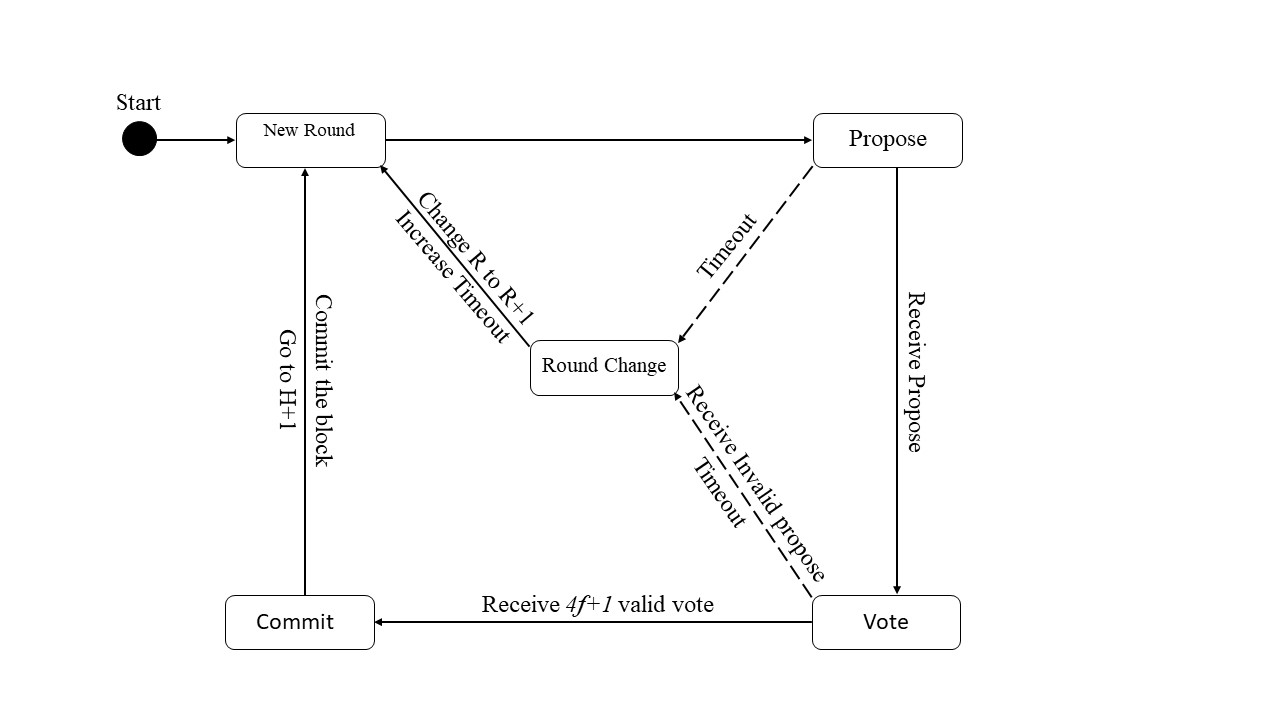
\includegraphics[scale=0.58]{images/2.jpg}
\caption{FaSBFT演算法流程圖}
\label{i:byz-latency}
\end{figure}
